\documentclass{standalone}
\usepackage{tikz}
\usetikzlibrary{patterns, positioning}
\usepackage[sfdefault]{ClearSans} %% option 'sfdefault' activates Clear Sans as the default text font
\usepackage[T1]{fontenc}

\begin{document}
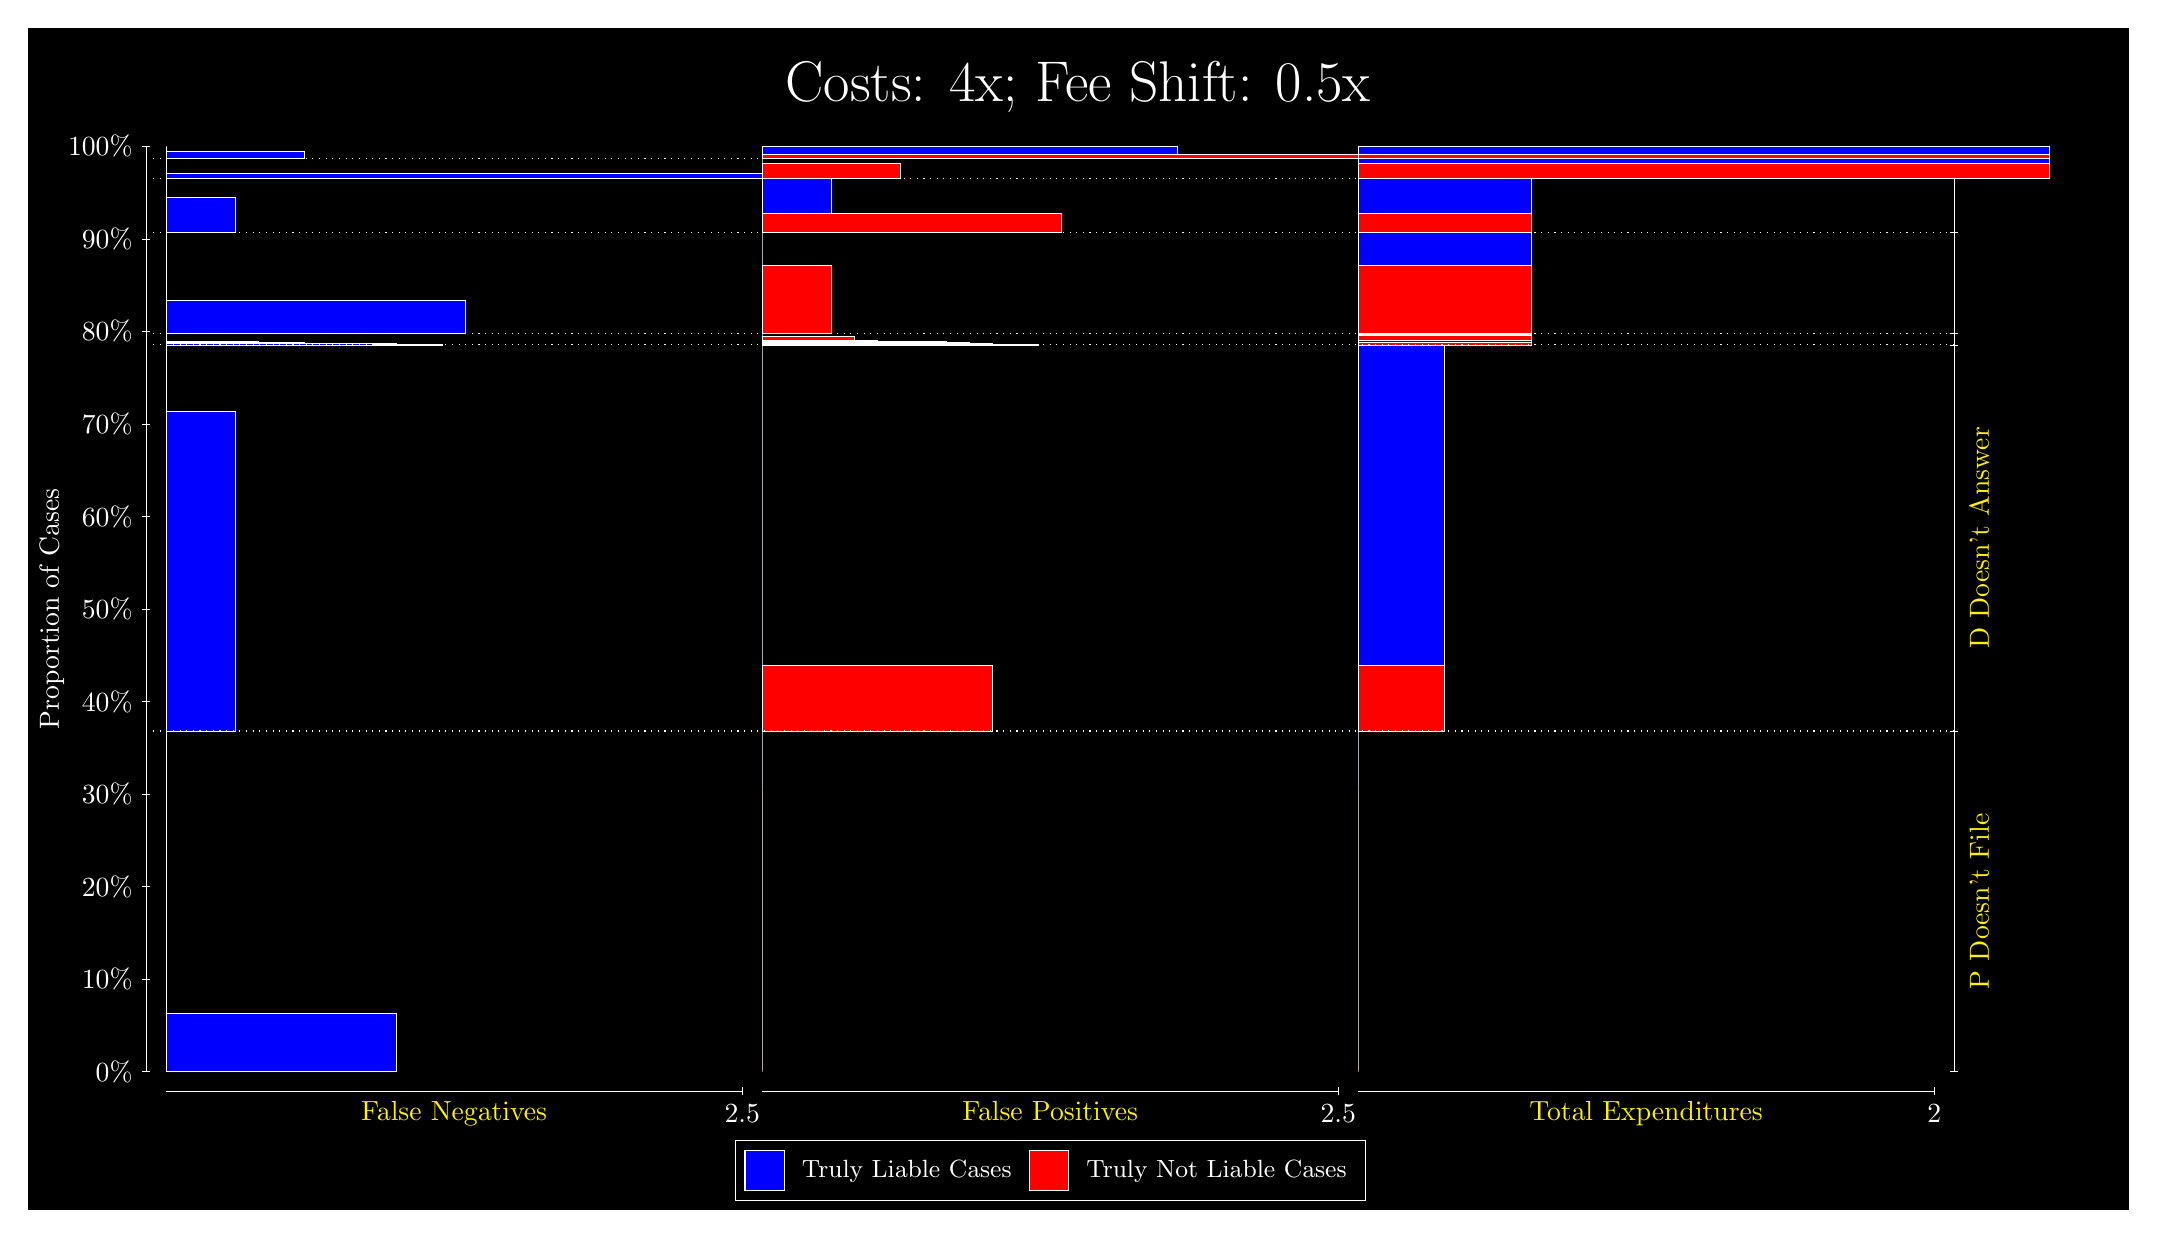
\begin{tikzpicture}
\draw[fill=black] (0,0) rectangle (26.667,15);
\draw[text=white] (0,13.5) rectangle (26.667,15) node[midway] {\huge Costs: 4x; Fee Shift: 0.5x};
\draw[white, very thin] (1.5,1.75) -- (1.5,13.5);
\node[rotate=90, text=white, anchor=center] at (0.3, 7.625) {Proportion of Cases};
\draw[white, very thin] (1.45,1.75) -- (1.55,1.75);
\node[text=white, anchor=east] at (1.45, 1.75) {0\%};
\draw[white, very thin] (1.45,2.925) -- (1.55,2.925);
\node[text=white, anchor=east] at (1.45, 2.925) {10\%};
\draw[white, very thin] (1.45,4.1) -- (1.55,4.1);
\node[text=white, anchor=east] at (1.45, 4.1) {20\%};
\draw[white, very thin] (1.45,5.275) -- (1.55,5.275);
\node[text=white, anchor=east] at (1.45, 5.275) {30\%};
\draw[white, very thin] (1.45,6.45) -- (1.55,6.45);
\node[text=white, anchor=east] at (1.45, 6.45) {40\%};
\draw[white, very thin] (1.45,7.625) -- (1.55,7.625);
\node[text=white, anchor=east] at (1.45, 7.625) {50\%};
\draw[white, very thin] (1.45,8.8) -- (1.55,8.8);
\node[text=white, anchor=east] at (1.45, 8.8) {60\%};
\draw[white, very thin] (1.45,9.975) -- (1.55,9.975);
\node[text=white, anchor=east] at (1.45, 9.975) {70\%};
\draw[white, very thin] (1.45,11.15) -- (1.55,11.15);
\node[text=white, anchor=east] at (1.45, 11.15) {80\%};
\draw[white, very thin] (1.45,12.325) -- (1.55,12.325);
\node[text=white, anchor=east] at (1.45, 12.325) {90\%};
\draw[white, very thin] (1.45,13.5) -- (1.55,13.5);
\node[text=white, anchor=east] at (1.45, 13.5) {100\%};

\draw[white, very thin] (24.457,1.75) -- (24.457,13.5);
\draw[white, very thin] (24.407,1.75) -- (24.507,1.75);
\node[anchor=west] at (24.407, 1.75) {};
\draw[white, very thin] (24.407,6.0744) -- (24.507,6.0744);
\node[anchor=west] at (24.407, 6.0744) {};
\draw[white, very thin] (24.407,10.978) -- (24.507,10.978);
\node[anchor=west] at (24.407, 10.978) {};
\draw[white, very thin] (24.407,11.127) -- (24.507,11.127);
\node[anchor=west] at (24.407, 11.127) {};
\draw[white, very thin] (24.407,12.403) -- (24.507,12.403);
\node[anchor=west] at (24.407, 12.403) {};
\draw[white, very thin] (24.407,13.097) -- (24.507,13.097);
\node[anchor=west] at (24.407, 13.097) {};
\draw[white, very thin] (24.407,13.343) -- (24.507,13.343);
\node[anchor=west] at (24.407, 13.343) {};
\draw[white, very thin] (24.407,13.5) -- (24.507,13.5);
\node[anchor=west] at (24.407, 13.5) {};

\draw[white, very thin, fill=blue] (1.75,1.75) rectangle (4.6775,2.4943);
\draw[white, very thin, fill=red] (1.75,2.4943) rectangle (1.75,6.0744);
\draw[white, very thin, fill=blue] (1.75,6.0744) rectangle (2.6283,10.139);
\draw[white, very thin, fill=red] (1.75,10.139) rectangle (1.75,10.978);
\draw[white, very thin, fill=blue] (1.75,10.978) rectangle (5.2631,10.989);
\draw[white, very thin, fill=blue] (1.75,10.989) rectangle (4.9703,10.991);
\draw[white, very thin, fill=blue] (1.75,10.991) rectangle (4.6775,10.993);
\draw[white, very thin, fill=blue] (1.75,10.993) rectangle (4.3848,10.993);
\draw[white, very thin, fill=blue] (1.75,10.993) rectangle (4.3848,10.994);
\draw[white, very thin, fill=blue] (1.75,10.994) rectangle (4.092,11.002);
\draw[white, very thin, fill=blue] (1.75,11.002) rectangle (3.7993,11.005);
\draw[white, very thin, fill=blue] (1.75,11.005) rectangle (3.5065,11.012);
\draw[white, very thin, fill=blue] (1.75,11.012) rectangle (3.2138,11.017);
\draw[white, very thin, fill=blue] (1.75,11.017) rectangle (2.921,11.019);
\draw[white, very thin, fill=red] (1.75,11.019) rectangle (1.75,11.127);
\draw[white, very thin, fill=blue] (1.75,11.127) rectangle (5.5558,11.543);
\draw[white, very thin, fill=red] (1.75,11.543) rectangle (1.75,12.403);
\draw[white, very thin, fill=blue] (1.75,12.403) rectangle (2.6283,12.854);
\draw[white, very thin, fill=red] (1.75,12.854) rectangle (1.75,13.097);
\draw[white, very thin, fill=blue] (1.75,13.097) rectangle (9.9471,13.156);
\draw[white, very thin, fill=red] (1.75,13.156) rectangle (1.75,13.343);
\draw[white, very thin, fill=blue] (1.75,13.343) rectangle (3.5065,13.441);
\draw[white, very thin, fill=red] (1.75,13.441) rectangle (1.75,13.5);
\draw[white, very thin, fill=red] (9.3189,1.75) rectangle (9.3189,5.33);
\draw[white, very thin, fill=blue] (9.3189,5.33) rectangle (9.3189,6.0744);
\draw[white, very thin, fill=red] (9.3189,6.0744) rectangle (12.246,6.9137);
\draw[white, very thin, fill=blue] (9.3189,6.9137) rectangle (9.3189,10.978);
\draw[white, very thin, fill=red] (9.3189,10.978) rectangle (12.832,10.98);
\draw[white, very thin, fill=red] (9.3189,10.98) rectangle (12.539,10.988);
\draw[white, very thin, fill=red] (9.3189,10.988) rectangle (12.246,11.002);
\draw[white, very thin, fill=red] (9.3189,11.002) rectangle (11.954,11.008);
\draw[white, very thin, fill=red] (9.3189,11.008) rectangle (11.661,11.02);
\draw[white, very thin, fill=red] (9.3189,11.02) rectangle (11.368,11.022);
\draw[white, very thin, fill=red] (9.3189,11.022) rectangle (11.075,11.029);
\draw[white, very thin, fill=red] (9.3189,11.029) rectangle (10.783,11.034);
\draw[white, very thin, fill=red] (9.3189,11.034) rectangle (10.49,11.086);
\draw[white, very thin, fill=blue] (9.3189,11.086) rectangle (9.9044,11.088);
\draw[white, very thin, fill=blue] (9.3189,11.088) rectangle (9.6116,11.093);
\draw[white, very thin, fill=blue] (9.3189,11.093) rectangle (9.3189,11.127);
\draw[white, very thin, fill=red] (9.3189,11.127) rectangle (10.197,11.987);
\draw[white, very thin, fill=blue] (9.3189,11.987) rectangle (9.3189,12.403);
\draw[white, very thin, fill=red] (9.3189,12.403) rectangle (13.125,12.646);
\draw[white, very thin, fill=blue] (9.3189,12.646) rectangle (10.197,13.097);
\draw[white, very thin, fill=red] (9.3189,13.097) rectangle (11.075,13.283);
\draw[white, very thin, fill=blue] (9.3189,13.283) rectangle (9.3189,13.343);
\draw[white, very thin, fill=red] (9.3189,13.343) rectangle (17.516,13.401);
\draw[white, very thin, fill=blue] (9.3189,13.401) rectangle (14.588,13.5);
\draw[white, very thin, fill=red] (16.888,1.75) rectangle (16.888,5.33);
\draw[white, very thin, fill=blue] (16.888,5.33) rectangle (16.888,6.0744);
\draw[white, very thin, fill=red] (16.888,6.0744) rectangle (17.986,6.9137);
\draw[white, very thin, fill=blue] (16.888,6.9137) rectangle (17.986,10.978);
\draw[white, very thin, fill=red] (16.888,10.978) rectangle (19.083,11.011);
\draw[white, very thin, fill=blue] (16.888,11.011) rectangle (19.083,11.032);
\draw[white, very thin, fill=red] (16.888,11.032) rectangle (19.083,11.096);
\draw[white, very thin, fill=blue] (16.888,11.096) rectangle (19.083,11.112);
\draw[white, very thin, fill=red] (16.888,11.112) rectangle (19.083,11.121);
\draw[white, very thin, fill=blue] (16.888,11.121) rectangle (19.083,11.127);
\draw[white, very thin, fill=red] (16.888,11.127) rectangle (19.083,11.987);
\draw[white, very thin, fill=blue] (16.888,11.987) rectangle (19.083,12.403);
\draw[white, very thin, fill=red] (16.888,12.403) rectangle (19.083,12.646);
\draw[white, very thin, fill=blue] (16.888,12.646) rectangle (19.083,13.097);
\draw[white, very thin, fill=red] (16.888,13.097) rectangle (25.67,13.283);
\draw[white, very thin, fill=blue] (16.888,13.283) rectangle (25.67,13.343);
\draw[white, very thin, fill=red] (16.888,13.343) rectangle (25.67,13.401);
\draw[white, very thin, fill=blue] (16.888,13.401) rectangle (25.67,13.5);
\draw[white, dotted] (1.5,6.0744) -- (24.457,6.0744);
\draw[white, dotted] (1.5,10.978) -- (24.457,10.978);
\draw[white, dotted] (1.5,11.127) -- (24.457,11.127);
\draw[white, dotted] (1.5,12.403) -- (24.457,12.403);
\draw[white, dotted] (1.5,13.097) -- (24.457,13.097);
\draw[white, dotted] (1.5,13.343) -- (24.457,13.343);
\draw[white, very thin] (1.75,1.5) -- (9.0689,1.5);
\node[text=yellow, anchor=north] at (5.4094, 1.5) {False Negatives};
\draw[white, very thin] (9.0689,1.45) -- (9.0689,1.55);
\node[text=white, anchor=north] at (9.0689, 1.45) {2.5};

\draw[white, very thin] (9.3189,1.5) -- (16.638,1.5);
\node[text=yellow, anchor=north] at (12.978, 1.5) {False Positives};
\draw[white, very thin] (16.638,1.45) -- (16.638,1.55);
\node[text=white, anchor=north] at (16.638, 1.45) {2.5};

\draw[white, very thin] (16.888,1.5) -- (24.207,1.5);
\node[text=yellow, anchor=north] at (20.547, 1.5) {Total Expenditures};
\draw[white, very thin] (24.207,1.45) -- (24.207,1.55);
\node[text=white, anchor=north] at (24.207, 1.45) {2};

\node[text=yellow, centered, rotate=90] at (24.777, 3.9122) {P Doesn't File};
\node[text=yellow, centered, rotate=90] at (24.777, 8.5262) {D Doesn't Answer};






\draw (12.978300999999998,1.5) node[draw=none] (baseCoordinate) {};
\begin{scope}[align=center]
        \matrix[scale=0.5, draw=white, below=0.5cm of baseCoordinate, nodes={draw}, column sep=0.1cm]{
            \node[rectangle, draw, minimum width=0.5cm, minimum height=0.5cm, fill=blue] {}; &
            \node[draw=none, font=\small, text=white] (B) {Truly Liable Cases}; &
            \node[rectangle, draw, minimum width=0.5cm, minimum height=0.5cm, fill=red] {}; &
            \node[draw=none, font=\small, text=white] (B) {Truly Not Liable Cases}; \\
            };
\end{scope}

\end{tikzpicture}
\end{document}